\documentclass{sig-alternate}
\usepackage{hyperref}
\usepackage{graphicx}
\usepackage{algorithm}
\usepackage[noend]{algorithmic}

\renewcommand{\algorithmicrequire}{\textbf{Input:}}
\renewcommand{\algorithmicensure}{\textbf{Output:}}
\newcommand{\FN}[1]{\leavevmode\hbox{\sc #1}}
\newcommand{\VAR}[1]{\leavevmode\hbox{\it #1\/}}

\newcommand{\todo}[1]{\par\framebox{\parbox{3in}{#1}}\par}
\newdimen\plotheight
\plotheight=3in

\begin{document}
%
% --- Author Metadata here ---
\conferenceinfo{K-CAP}{2015 Palisades, NY, USA}
%\CopyrightYear{2007} % Allows default copyright year (20XX) to be over-ridden - IF NEED BE.
%\crdata{0-12345-67-8/90/01}  % Allows default copyright data (0-89791-88-6/97/05) to be over-ridden - IF NEED BE.
% --- End of Author Metadata ---

\title{Dynamically Time-Capped Possibilistic Testing of OWL Axioms Against RDF Data}
%\titlerunning{Time-Capped Testing of OWL Axioms}

\numberofauthors{3}

\author{
%
% The command \alignauthor (no curly braces needed) should
% precede each author name, affiliation/snail-mail address and
% e-mail address. Additionally, tag each line of
% affiliation/address with \affaddr, and tag the
% e-mail address with \email.
%
\alignauthor
Andrea G. B. Tettamanzi\\
  \affaddr{Univ. Nice Sophia Antipolis, I3S, UMR 7271}\\
  \affaddr{Sophia Antipolis, France}\\
  \email{andrea.tettamanzi@unice.fr}
\alignauthor
Catherine Faron Zucker\\
  \affaddr{Univ. Nice Sophia Antipolis, I3S, UMR 7271}\\
  \affaddr{Sophia Antipolis, France}\\
  \email{faron@unice.fr}
\alignauthor
Fabien Gandon\\
  \affaddr{INRIA Sophia Antipolis -- M\'editerran\'ee}\\
  \affaddr{Sophia Antipolis, France}\\
  \email{fabien.gandon@inria.fr}
}

\maketitle

\begin{abstract}
Axiom scoring is a critical task both for the automatic enrichment/learning
and for the automatic validation of knowledge bases and ontologies.
We develop an axiom scoring heuristics based on possibility theory,
which aims at overcoming some limitations of scoring heuristics based on statistical inference
and working with an open-world semantics.
Since computing the possibilistic score can be computationally quite heavy
for some candidate axioms, we propose a method based on time capping
to alleviate the computation of the heuristics without giving up the precision of the scores.
We evaluate our proposal by applying it to the problem of testing \textsf{SubClassOf}
axioms against the DBpedia RDF dataset.
\end{abstract}

\keywords{ontology learning, open-world assumption, possibility theory}

\section{Introduction}

It is common practice, in the semantic Web, to put a strong emphasis
on the construction or reuse of ontologies based on a principled conceptual analysis
of a domain of interest, as a prerequisite for the organization of the Linked Open Data (LOD),
much like a database schema must be designed before a database can be populated.
While this approach is quite successful when applied to specific domains,
it does not scale well to more general settings;
it is aprioristic and dogmatic;
it does not lend itself to a collaborative effort; etc.
That is why an alternative, bottom-up, \emph{grass-roots} approach to ontology and
knowledge base creation better suits many scenarios: instead of postulating an \emph{a priori}
conceptualization of reality (i.e., an ontology) and requiring that our knowledge
about facts complies with it, one can start from RDF facts and learn OWL~2 axioms.

Recent contributions towards the automatic creation of OWL~2 ontologies
from large repositories of RDF facts include
FOIL-like algorithms for learning concept definitions~\cite{FanizziDAmatoEsposito2008},
statistical schema induction via association rule mining~\cite{FleischhackerVoelkerStuckenschmidt2012},
and light-weight schema enrichment methods based on the DL-Learner
framework~\cite{HellmannLehmannAuer2009,BuehmannLehmann2012}.
All these methods apply and extend techniques developed within inductive logic programming
(ILP)~\cite{ILPat20}. For a recent survey of the wider field of ontology learning,
see~\cite{LehmannVoelker2014}.

On a related note, there exists a need for evaluating and validating ontologies,
be they the result of an analysis effort or of a semi-automatic learning method.
This need is witnessed by general methodological investigations
\cite{GangemiCatenacciCiaramitaLehmann2005,GangemiCatenacciCiaramitaLehmann2006}
and surveys \cite{TartirBudakArpinarSheth2007} and tools like OOPS! \cite{PovedaSuarezGomez2012}
for detecting pitfalls in ontologies.

Ontology engineering methodologies, such as METHONTOLOGY~\cite{FernandezGomezJuristo1997},
distinguish two validation activities, namely verification (through formal methods, syntax, logics, etc.)
and validation through usage. Whilst this latter is usually thought of as user studies,
an automatic process of validation based on RDF data would provide a cheap alternative,
whereby the existing linked data may be regarded as usage traces that can be used
to test and improve the ontologies, much like log mining can be used to provide
test cases for development in the replay approaches.
Alternatively, one may regard the ontology as a set of integrity constraints and check if the
data satisfy them, using a tool like Pellet integrity constraint validator (ICV),
which translates OWL ontologies into SPARQL queries to automatically validate RDF data~\cite{SirinTao2009}.
A similar approach also underlies the idea of test-driven evaluation of linked data 
quality~\cite{KontokostasWestphalAuerHellmannLehmannCornelissen2014}.
To this end, OWL ontologies are interpreted under the closed-world assumption and
the weak unique name assumption. 

Yet this validation process may be seen from a reverse point of view:
instead of starting from the \emph{a priori} assumption that a given ontology
is correct and verify whether the facts contained in an RDF base satisfy it,
one may treat ontologies like hypotheses and develop a methodology to verify
whether the RDF facts corroborate or falsify them. Ontology learning and validation
are thus strictly related.
They could even be seen as an agile and test-driven approach to ontology development,
where the linked data is used as a giant test case library not only to validate the
schema but even to suggest new developments.

Ontology learning and validation rely critically on (candidate) axiom scoring.
In this paper, we will tackle the problem of testing a single, isolated axiom,
which is anyway the first step to solve the problem of validating an entire ontology.
Furthermore, to keep things reasonably simple, we will restrict our attention
to subsumption axioms of the form $\mathsf{SubClassOf}(C\ D)$.

The most popular scoring heuristics proposed in the literature are based on statistical inference.
We argue that such a probability-based framework is not always completely satisfactory.
We propose an axiom scoring heuristics based on a formalization in possibility theory of
the notions of logical content of a theory and of falsification, loosely inspired
by Karl Popper's approach to epistemology, and working with an open-world semantics.

Some preliminary results~\cite{TettamanziFaronZuckerGandon2014ekaw} indicate that
applying a possibilistic approach to the task of testing candidate axioms
for ontology learning yields very promising results and hints that the same approach
could be beneficial to ontology and knowledge base validation as well.
At the same time, the proposed heuristics is much heavier, from a computational
point of view, than the probabilistic scores it aims to complement.
Fortunately, there is evidence (see~\cite{TettamanziFaronZuckerGandon2014ekaw} and
Section~\ref{evaluation} below) that the time it takes to test an axiom
tends to be inversely proportional to its score.
This suggests that time-capping the test might be an acceptable additional heuristics
to decide whether to accept or reject a candidate axiom, for an axiom which takes
too long to test will likely end up having a very negative score.
In this paper, we follow this suggestion and investigate the effectiveness
of time-capped possibilistic testing of OWL axioms against the facts contained
in an RDF repository.
Our research question is, therefore: ``Can time capping alleviate the computation
of the proposed possibilistic axiom scoring heuristics without giving up
the precision of the scores?''
This paper is organized as follows: \todo{Paper structure}

\section{Principles of Axiom Testing}\label{principles}

Testing an axiom against an RDF dataset can be done by checking whether the formulas entailed by it
are confirmed by the facts contained in the RDF dataset.\footnote{Note that calling linked data search engines
like Sindice could virtually extend the dataset to the whole LOD cloud.}

\subsection{Direct Model-Theoretic Semantics for OWL 2}
We refer to the model-theoretic semantics of OWL~2 as defined in~\cite{OWL2-direct-semantics}.\footnote{\url{http://www.w3.org/TR/2012/REC-owl2-direct-semantics-20121211/}, Section 2.2 Interpretations}
An interpretation $\mathcal{I}$ for a datatype map $D$ and a vocabulary $V$ over $D$ is defined by an interpretation domain $\Delta^\mathcal{I}=\Delta_{I}\cup\Delta_{D}$  ($\Delta_{I}$ is the \textit{object domain} and $\Delta_{D}$ the \textit{data domain}), and a valuation function $\cdot^{\mathcal{I}}$ with seven restrictions: $\cdot^{C}$ mapping class expressions to subsets of $\Delta_{I}$,  $\cdot^{OP}$ mapping object properties to subsets of $\Delta_{I}\times\Delta_{I}$, $\cdot^{DP}$ mapping data properties to subsets of $\Delta_{I}\times\Delta_{D}$, $\cdot^{I}$ mapping individuals to elements of $\Delta_{I}$, $\cdot^{DT}$ mapping datatypes to subsets of $\Delta_{D}$, $\cdot^{LT}$ mapping literals to elements of the set of data values $(DT)^{DT}$ of $D$ and $\cdot^{FT}$ mapping facets to subsets of $(DT)^{DT}$.
% REVOIR DÉFINITION DE $\Delta^\mathcal{I}$
%Testing an axiom amounts to constructing an interpretation $\mathcal{I}$ compatible
%with the available data and testing whether $\mathcal{I}$ is a model of the axiom.
%We take the set of all the resources and literal values that occur in a given RDF store 
%as $\Delta^\mathcal{I}$.
%reviewer 5: Not true, there could be un-named individuals in the interpretation domain.

\subsection{Content, Support, Confirmation, and Counterexample of an Axiom}
 
Let $\phi$ be a candidate axiom; we denote by $u_\phi$ the support of $\phi$,
i.e., the cardinality of the set of formulas entailed by $\phi$ which will be tested
against the facts contained in the RDF dataset.
We shall define this notion of support with respect to an RDF dataset more precisely.

%Let $gp(\mathtt{?x})$ and $gp(\mathtt{?x}, \mathtt{?y})$ be SPARQL graph patterns
%where variables \texttt{?x} and \texttt{?y} occur (other variables may occur as well)
%and let $[gp(\mathtt{?x})]$ and $[gp(\mathtt{?x}, \mathtt{?y})]$ denote
%the set of values bound to variable \texttt{?x} in the result set of SPARQL query
%\texttt{SELECT ?x WHERE} \{ $gp(\mathtt{?x})$ \} and
%the set of value pairs bound to variables \texttt{?x} and \texttt{?y} in the result set of SPARQL query
%\texttt{SELECT ?x ?y WHERE} \{ $gp(\mathtt{?x}, \mathtt{?y})$ \}, respectively.

We define the \emph{content} of an axiom $\phi$, $content(\phi)$, as the finite set of formulas,
which can be tested against an RDF dataset $\mathcal{K}$,
constructed from the set-theoretic formulas expressing the semantics of $\phi$
by grounding them, i.e., by
\begin{itemize}
\item omitting all $\forall$ quantifiers,
\item substituting all universally quantified variable symbols $x$ denoting an individual
of $\Delta^\mathcal{I}$ by every resource $r$ or literal $l$ occurring in $\mathcal{K}$,%
\footnote{This may be construed as $r^\mathcal{I} = x$ or $l^\mathcal{I} = x$}
\item substituting all symbols $C^\mathcal{I}$ denoting subsets of $\Delta^\mathcal{I}$
by their corresponing class name or datatype name $C$, and
\item substituting all symbols $R^\mathcal{I}$ denoting subsets of $\Delta_{I}\times\Delta_{I}$ or $\Delta_{I}\times\Delta_{D}$
by their corresponding object or data property name $R$.
\end{itemize}
For example, let us consider the test of candidate axiom
\[
  \phi = \mbox{\texttt{SubClassOf}(\texttt{dbo:LaunchPad} \texttt{dbo:Infrastructure})},
\]
or $\mbox{\tt dbo:LaunchPad} \sqsubseteq \mbox{\tt dbo:Infrastructure}$
in Description Logics (DL) syntax, against the DBpedia dataset.
The semantics of $\phi$ is
\[
  \mbox{\texttt{dbo:LaunchPad}}^\mathcal{I} \subseteq \mbox{\texttt{dbo:Infrastructure}}^\mathcal{I},
\]
which can also be written as
\[
  \forall x \in \Delta^\mathcal{I},
  x \in \mbox{\texttt{dbo:LaunchPad}}^\mathcal{I} \Rightarrow x \in \mbox{\texttt{dbo:Infrastructure}}^\mathcal{I}.
\]
We may thus express $content(\phi)$ as
\[
  \begin{array}{rrl}
    \{ & \mbox{\tt dbo:LaunchPad}(r) \Rightarrow \mbox{\tt dbo:Infrastructure}(r) : &\\
       & \mbox{$r$ is a resource occurring in DBPedia} & \}.
  \end{array}
\]
By construction, for all $\psi \in content(\phi)$, $\phi \models \psi$.
Indeed, let $\mathcal{I}$ be a model of $\phi$;
by definition, $\mathcal{I}$ is also a model of the formula which expresses the semantics of $\phi$
and \emph{a fortiori}, also of all its groundings; since $\psi$ is a grounding of the
formula which expresses the semantics of $\phi$, $\mathcal{I}$ is a model of $\psi$.

Now, given a formula $\psi \in content(\phi)$ and an RDF dataset $\mathcal{K}$,
there are three cases:
\begin{enumerate}
\item $\mathcal{K} \models \psi$:
  in this case, we will call $\psi$ a \emph{confirmation} of $\phi$;
\item $\mathcal{K} \models \neg\psi$:
  in this case, we will call $\psi$ a \emph{counterexemple} of $\phi$;
\item $\mathcal{K} \not\models \psi$ and $\mathcal{K} \not\models \neg\psi$:
  in this case, $\psi$ is neither a confirmation nor a counterexample of $\phi$.
\end{enumerate}

The definition of $content(\phi)$ may be refined by adopting Scheffler and Goodman's principle of
\emph{selective confirmation}~\cite{SchefflerGoodman1972},
which characterizes a confirmation as a fact not simply confirming a candidate axiom, but, further,
favoring the axiom rather than its contrary.
For instance, the occurence of a black raven \emph{selectively confirms} the axiom
$\mathtt{Raven} \sqsubseteq \mathtt{Black}$ because it both confirms it and fails to confirm its
negation, namely that there exist ravens that are not black. On the contrary, the observation of
a green apple does not contradict $\mathtt{Raven} \sqsubseteq \mathtt{Black}$,
but it does not disconfirm $\mathtt{Raven} \not\sqsubseteq \mathtt{Black}$
either, i.e., it does not selectively confirm $\mathtt{Raven} \sqsubseteq \mathtt{Black}$.


The definition of $content(\phi)$ may be further refined, in order to restrict it
just to those $\psi$ which can be counterexamples of $\phi$,
thus leaving out all those $\psi$ which would be trivial confirmations of $\phi$.
That is like saying that, to test a hypothesis, we have to try, as hard as we can,
to refute it.

For example, in the case of a $\mathtt{SubClassOf}(C\ D)$ axiom,
all $\psi$ involving the existence of a resource $r$ for which $\mathcal{K} \not\models C(r)$
will either be confirmations (if $\mathcal{K} \models D(r)$) or they
will fall into Case~3 otherwise. Therefore, such $\psi$ will not be interesting
and should be left out of $content(\mathtt{SubClassOf}(C\ D))$.

%\todo{définir content en général et pas seulement pour subclass?}


Applying this principle greatly reduces $content(\phi)$ and, therefore,
the number of $\psi$ that will have to be checked.



We can now define the support of $\phi$ as the cardinality of $content(\phi)$:
\begin{equation}\label{eq:support}
    u_\phi = \|content(\phi)\|.
\end{equation}
Since an RDF dataset is finite, $u_\phi$ is also finite.
%\noindent
%For the axiom $C \sqsubseteq D$, $u_{C \sqsubseteq D} = \|C^\mathcal{I}\|$.

We denote by $u_\phi^+$ the number of formulas $\psi \in content(\phi)$
which are entailed by the RDF dataset (confirmations);
and by $u_\phi^-$ the number of such formulas
whose negation $\neg\psi$ is entailed by the RDF dataset (counterexamples).
Notice that it is possible that, for some $\psi \in content(\phi)$,
the RDF dataset entails neither $\psi$ nor $\neg\psi$ (Case~3 above). Therefore,
\begin{equation}
  u_\phi^+ + u_\phi^- \leq u_\phi.\label{eq:conf-pls-expt-lt-refc}
\end{equation}
For example, when testing
\[
  \phi = \mbox{\tt dbo:LaunchPad} \sqsubseteq \mbox{\tt dbo:Infrastructure}
\]
against the DBpedia dataset, we found that $u_\phi = 85$,
$u_\phi^+ = 83$, i.e., there are 83 confirmations of $\phi$ in the dataset; 
and $u_\phi^- = 1$, i.e., there is 1 couterexample in the dataset, namely
\[
  \mbox{\tt dbo:LaunchPad}(\mbox{\tt :USA}) \Rightarrow
  \mbox{\tt dbo:Infrastructure}(\mbox{\tt :USA}),
\]
since
\begin{eqnarray*}
  \mbox{DBpedia} &\models& \mbox{\tt dbo:LaunchPad}(\mbox{\tt :USA}),\\
  \mbox{DBpedia} &\models& \neg\mbox{\tt dbo:Infrastructure}(\mbox{\tt :USA}).
\end{eqnarray*}
and one formula in $content(\phi)$ is neither a confirmation nor a counterexample, namely
\[
  \begin{array}{l}
    \mbox{\tt dbo:LaunchPad}(\mbox{\tt :Cape\_Canaveral}) \Rightarrow\\
    \mbox{\tt dbo:Infrastructure}(\mbox{\tt :Cape\_Canaveral}),
  \end{array}
\]
because
\begin{eqnarray*}
  \mbox{DBpedia} &\models& \mbox{\tt dbo:LaunchPad}(\mbox{\tt :Cape\_Canaveral}),\\
  \mbox{DBpedia} &\not\models& \mbox{\tt dbo:Infrastructure}(\mbox{\tt :Cape\_Canaveral}),\\
  \mbox{DBpedia} &\not\models& \neg\mbox{\tt dbo:Infrastructure}(\mbox{\tt :Cape\_Canaveral}).
\end{eqnarray*}


Further interesting properties of $u_\phi$, $u^+_\phi$, and $u^-_\phi$ are the following:
\begin{enumerate}
\item $u_\phi^+ = u_{\neg\phi}^-$ (the confirmations of $\phi$ are counterexamples of $\neg\phi$);
\item $u_\phi^- = u_{\neg\phi}^+$ (the counterexamples of $\phi$ are confirmations of $\neg\phi$);
\item $u_\phi = u_{\neg\phi}$ ($\phi$ and $\neg\phi$ have the same support).
\end{enumerate}


\section{A Possibilistic Candidate Axiom Scoring}
\label{possibility-theory}

We present an axiom scoring heuristics which captures the basic intuition
behind the process of axiom discovery based on possibility theory: assigning to a candidate axiom a degree of possibility equal to 1 just means that this axiom is possible, plausible, i.e. is not contradicted by facts in the knowledge base. This is  much weaker than assigning a probability equal to 1, meaning that the candidate axiom certainly \textit{is} an axiom.

\subsection{Possibility Theory}

Possibility theory~\cite{Zadeh1978} is a mathematical theory of epistemic uncertainty.
Given a finite universe of discourse $\Omega$, whose elements $\omega\in\Omega$
may be regarded as events, values of a variable, possible worlds, or states of affairs,
a possibility distribution is a mapping $\pi: \Omega \to [0, 1]$,
which assigns to each $\omega$ a degree of possibility ranging from 0 (impossible,
excluded) to 1 (completely possible, normal).
A possibility distribution $\pi$ for  which there exists a completely possible state of
affairs ($\exists \omega \in \Omega: \pi(\omega) = 1$) is said to be \emph{normalized}.

There is a similarity between possibility distribution and probability 
density. However, it must be stressed that $\pi(\omega) = 1$ just means that
$\omega$ is a plausible (normal) situation and therefore should not be excluded.
A degree of possibility can then be viewed as an upper bound of a degree of probability.
See~\cite{dubois1991} for a discussion
about the relationships between fuzzy sets, possibility, and probability 
degrees.
Possibility theory is suitable to represent incomplete knowledge while 
probability is adapted to represent random and observed phenomena. 


A possibility distribution $\pi$ induces a \emph{possibility
measure}\index{possibility measure} and its dual \emph{necessity
measure}\index{necessity measure}, denoted by $\Pi$ and $N$
respectively. Both measures apply to a set $A \subseteq\Omega$ (or to a
formula $\phi$, by way of the set of its models, $A = \{\omega : \omega \models \phi\}$),
and are defined as follows:
\begin{eqnarray}
  \Pi(A) &=& \max_{\omega\in A} \pi(\omega); \\
  N(A)   &=& 1 - \Pi(\bar{A}) = \min_{\omega\in \bar{A}} \{1 - \pi(\omega)\}.
\end{eqnarray}
%In words, the possibility measure of $A$ corresponds to the
%greatest of the possibilities associated to its elements; conversely,
%the necessity measure of $A$ is equivalent to the impossibility of
%its complement $\bar{A}$.
%
Here are a few properties of possibility and necessity measures 
induced by a normalized possibility distribution on a finite universe of
discourse $\Omega$: 

\begin{enumerate}
%  \item $\Pi(A \cup B) = \max\{\Pi(A), \Pi(B)\}$;
%  \item $\Pi(A \cup \bar A) = \max\{\Pi(A), \Pi(\bar A)\}=1$;
  \item $\Pi(\emptyset) = N(\emptyset) = 0$,\quad $\Pi(\Omega) = N(\Omega) = 1$;
%  \item $N(A \cap B) = \min\{N(A), N(B)\}$;
  \item $\forall A\subseteq \Omega,$ $\Pi(A) = 1 - N(\bar{A})$ (duality);
%  \item $N(A) \leq \Pi(A)$;
  \item $\forall A\subseteq \Omega$, $N(A) > 0$ implies $\Pi(A) = 1$, and $\Pi(A) < 1$ implies $N(A) = 0$.
\end{enumerate}
In case of complete ignorance on $A$, $\Pi(A) = \Pi(\bar{A}) = 1$.


\subsection{Possibility and Necessity of an Axiom}

The basic principle for establishing the possibility of a formula $\phi$ should be
that the absence of counterexamples to $\phi$ in the RDF repository means $\Pi(\phi) = 1$,
i.e., that $\phi$ is completely possible.

A hypothesis should be regarded as all the more
\emph{necessary} as it is explicitly supported by facts and not contradicted by any fact;
and all the more \emph{possible} as it is not contradicted by facts.
In other words, given hypothesis $\phi$, $\Pi(\phi) = 1$ if no counterexamples are found; 
as the number of counterexamples increases, $\Pi(\phi) \to 0$ strictly monotonically;
$N(\phi) = 0$ if no confirmations are found; as the number of confirmations increases
and no counterexamples are found, $N(\phi) \to 1$ strictly monotonically.
Notice that a confirmation of $\phi$ is a counterexample of $\neg\phi$
and that a counterexample of $\phi$ is a confirmation of $\neg\phi$.

Here are a few postulates the possibility
and necessity functions should obey:
\begin{enumerate}
\item $\Pi(\phi) = 1$ if $u_\phi^- = 0$;
\item $N(\phi) = 0$ if $u_\phi^- > 0$ or $u_\phi^+ = 0$;
\item let $u_\phi = u_\psi$; then $\Pi(\phi) > \Pi(\psi)$ iff $u_\phi^- < u_\psi^-$;
\item let $u_\phi = u_\psi$; then $N(\phi) > N(\psi)$ iff $u_\phi^+ > u_\psi^+$ and $u_\phi^- = 0$;
\item let $u_\phi = u_\psi = u_\chi$ and let $u_\psi^- < u_\phi^- < u_\chi^-$: then
  \[
    \frac{\Pi(\psi) - \Pi(\phi)}{u_\phi^- - u_\psi^-} > \frac{\Pi(\phi) - \Pi(\chi)}{u_\chi^- - u_\phi^-},
  \]
  i.e., the first counterexamples found to an axiom should determine a sharper decrease
  of the degree to which we regard the axiom as possible than any further counterexamples,
  because these latter will only confirm our suspicions and, therefore, will provide
  less and less information;
\item let $u_\phi = u_\psi = u_\chi$ and $u_\psi^- = u_\phi^- = u_\chi^- = 0$,
  and let $u_\psi^+ < u_\phi^+ < u_\chi^+$: then
  \[
    \frac{N(\phi) - N(\psi)}{u_\phi^+ - u_\psi^+} > \frac{N(\chi) - N(\phi)}{u_\chi^+ - u_\phi^+},
  \]
  i.e., in the absence of counterexamples,
  the first confirmations found to an axiom should determine a sharper increase
  of the degree to which we regard the axiom as necessary than any further confirmations,
  because these latter will only add up to our acceptance and, therefore, will provide
  less and less information.% (cf.~\cite{Popper1935}, \S83).
\end{enumerate}

Definitions of $\Pi$ and $N$ which satisfy the above postulates are, for $u_\phi > 0$,
%cath dans une version longue il faudrait le montrer
\begin{eqnarray}
  \label{eq:possibility}
  \Pi(\phi) &=& 1 - \sqrt{1 - \left(\frac{u_\phi - u_\phi^-}{u_\phi}\right)^2}; \\
  \label{eq:necessity}
  N(\phi) &=& \left\{\begin{array}{ll}
    \sqrt{1 - \left(\frac{u_\phi - u_\phi^+}{u_\phi}\right)^2},\quad & \mbox{if $u_\phi^- = 0$,}\\[1.5em]
    0, & \mbox{if $u_\phi^- > 0$.}
  \end{array}\right.
\end{eqnarray}
Notice that this is by no means the only possible definition, but 
it is the simplest one (it derives from a quadratic equation; a linear equation would
not satisfy all the postulates).
%cath dans une version longue il faudrait le montrer

%Figure~\ref{fig:poss-nec-plots} shows $\Pi(\phi)$ and $N(\phi)$ as a function of
%$u_\phi^-$ and $u_\phi^+$, respectively.
% The two functions describe an arc of an ellipse between the minor and the major axis.
It may be shown that the above definition satisfies the duality of
possibility and necessity, in that $N(\phi) = 1 - \Pi(\neg\phi)$ and
$\Pi(\phi) = 1 - N(\neg\phi)$.
As a matter of fact, we will seldom be interested in computing the necessity and
possibility degrees of the negation of OWL~2 axioms, for the simple reason that, in most cases,
the latter are not OWL~2 axioms themselves. For instance, while $C \sqsubseteq D$
is an axiom, $\neg(C \sqsubseteq D) = C \not\sqsubseteq D$ is not.
%Fabien true, but we will have to search and see if there were discussions on the NegativeObjectPropertyAssertion of OWL2 which is limited to IndividualAxiom for now ; just in case.


%\begin{figure}[t]
%  \begin{center}
%    \begin{tabular}{cc}
%      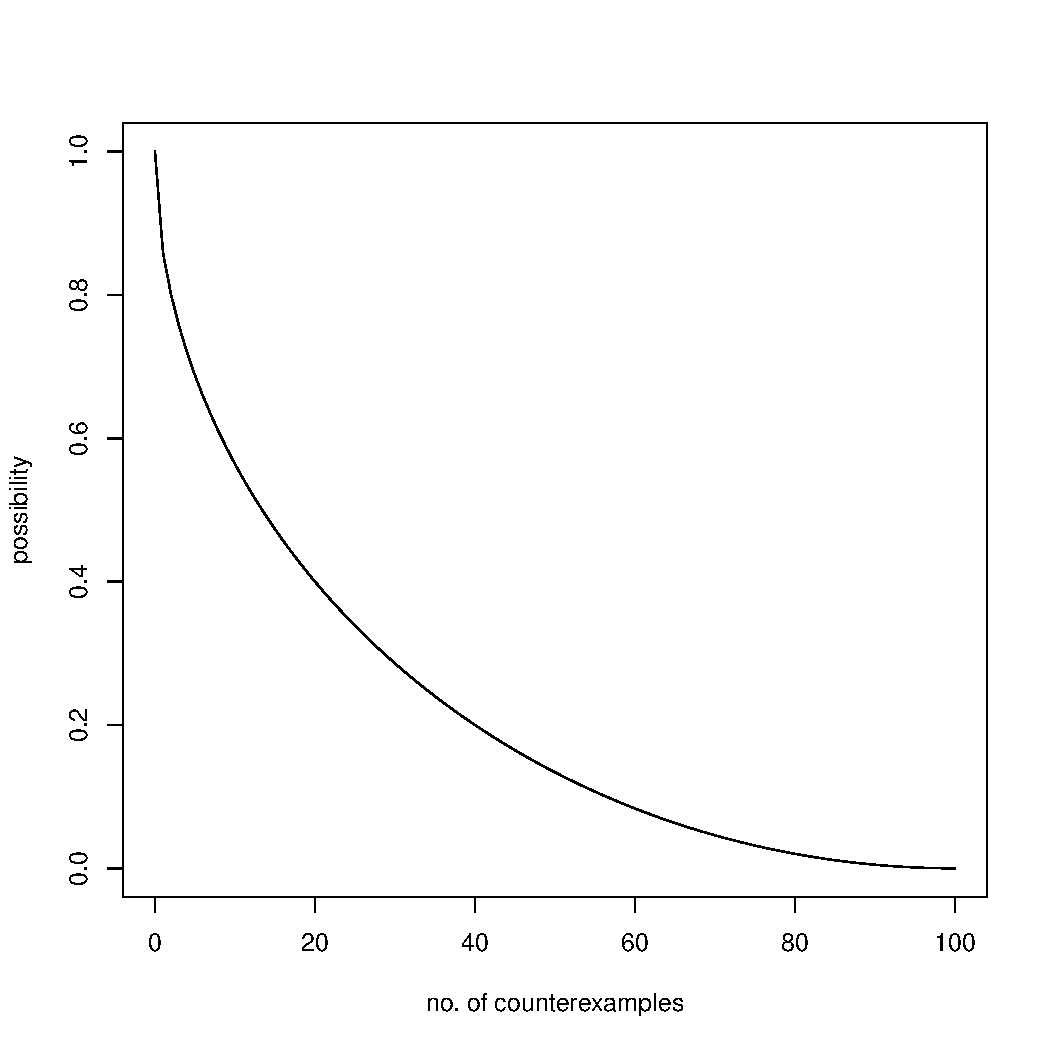
\includegraphics[width=\plotheight]{../possibility} &
%      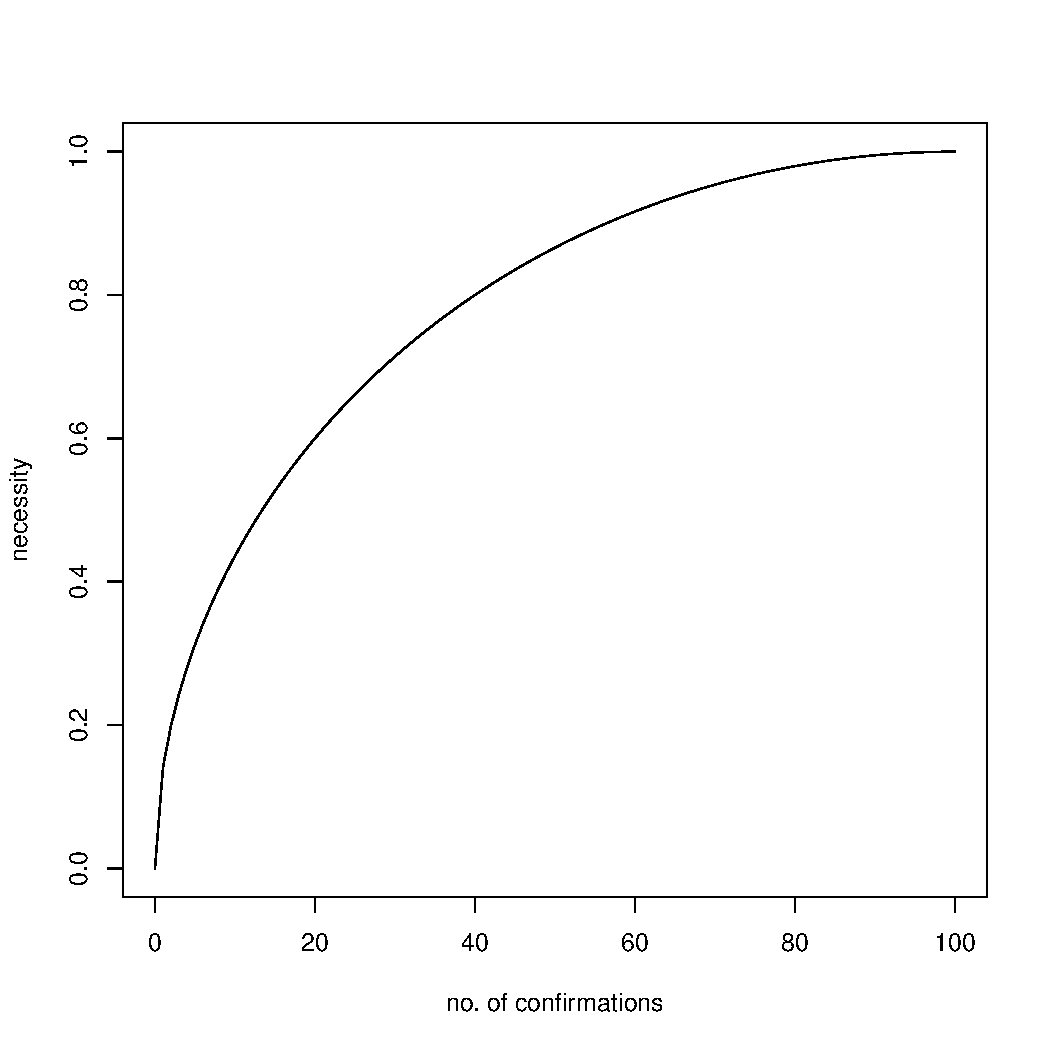
\includegraphics[width=\plotheight]{../necessity} \\
%      (a) & (b)
%    \end{tabular}
%  \end{center}
%  \caption{A plot of $\Pi(\phi)$  as a function of
%    $u_\phi^-$ (a) and of $N(\phi)$ as a function of
%    $u_\phi^+$ (b) when $u_\phi = 100$.\label{fig:poss-nec-plots}}
%\end{figure}

\subsection{Axiom Scoring}
We combine the possibility and necessity of an axiom to define
a single handy acceptance/rejection index (ARI) as follows:
\begin{equation}\label{eq:ARI}
  \mathrm{ARI}(\phi) = N(\phi) - N(\neg\phi) = N(\phi) + \Pi(\phi) - 1 \in [-1, 1].
\end{equation}
A negative $\mathrm{ARI}(\phi)$ suggests rejection of $\phi$ ($\Pi(\phi)<1$),
whilst a positive $\mathrm{ARI}(\phi)$ suggests its acceptance ($N(\phi)>0$),
with a strength proportional to its absolute value. A value close to zero
reflects ignorance about the status of $\phi$.

Although this ARI is useful for the purpose of analyzing the results of our
experiments and to visualize the distribution of the tested axiom with respect
to a single axis, one should always bear in mind that an axiom is scored by
the proposed heuristics in terms of two bipolar figures of merit,
whose meanings, though related, are very different:
\begin{itemize}
\item $\Pi(\phi)$ expresses the degree to which $\phi$ may be considered ``normal'',
  in the sense of ``not exceptional, not surprising'', or not contradicted by
  actual observations;
\item $N(\phi)$, on the other hand, expresses the degree to which $\phi$ is
  certain, granted by positive evidence and corroborated by actual observations.
\end{itemize}


\section{A Framework for Candidate Axiom Testing}
\label{OWL2SPARQL} 



%The semantics of the 32 axiom types of OWL~2 may be taken as a starting point to define,
%for each axiom type, which facts recorded in a given RDF triple store are to be taken as
%supporting evidence, or \emph{confirmations} of the axiom and which facts are to be
%construed as refuting evidence, or \emph{counterexamples}, based on the principles
%laid out in Section~\ref{epistemology}.

A general algorithm for testing all the possible OWL~2 axioms in a given RDF store is beyond the scope of this paper. 
Here, we will restrict our attention to \texttt{Class} and \texttt{ObjectComplementOf} class expressions and to \texttt{SubClassOf} axioms. 
Scoring these axioms with their ARI requires to compute the interpretation of \texttt{Class} and \texttt{ObjectComplementOf} class expressions. 
 
\subsection{Computational Definition of \texttt{Class} and \texttt{ObjectComplementOf} Class Expressions}
We define a mapping $Q(E, \mbox{\tt ?x})$ from OWL~2 class expressions to SPARQL graph patterns,
where $E$ is an OWL~2 class expression, and $\mbox{\tt ?x}$ is a variable,
such that the query
\texttt{SELECT DISTINCT ?x WHERE \{} $Q(E, \mbox{\tt ?x})$ \texttt{\}}
returns all the individuals which are instances of $E$. We denote this set by
$[Q(E, \mbox{\tt ?x})]$:
\begin{equation}
  \begin{array}{rcl}
    [Q(E, \mbox{\tt ?x})] &=& \{ v : (?x, v) \in ResultSet(\mbox{\tt SELECT}\\
                          & & \mbox{\tt\ DISTINCT ?x WHERE} \{ Q(E, \mbox{\tt ?x}) \} \}.
  \end{array}
\end{equation} 

For a \texttt{Class} class expression $A$ (i.e., an atomic concept in DL), 
\begin{equation}
Q(A, \mbox{\tt ?x}) = \{\mbox{\tt ?x a }A \},
\end{equation}
where $A$ is a valid IRI.

For an \texttt{ObjectComplementOf} class expression, things are slightly more complicated, since RDF does not support
negation. The model-theoretic semantics of OWL class expressions of the form \texttt{ObjectComplementOf(}$C$\texttt{)}
($\neg C$ in DL syntax), where $C$ denotes a class, is $\Delta^\mathcal{I} \setminus C^\mathcal{I}$.
However, to learn axioms from an RDF dataset, the open-world hypothesis must be made: the absence of
supporting evidence does not necessarily contradict an axiom, moreover an axiom might
hold even in the face of a few counterexamples.
%For example, for 143 out of 541 \texttt{SubClassOf} axioms in the DBpedia
%ontology, no resource in the DBpedia dataset provides any evidence;
%for 28, at least one counterexample is found in DBpedia 3.9.
%Axiom \texttt{SubClassOf(dbo:Person dbo:Agent)} even has 76 counterexamples!
%\todo{voir si on veut virer le paragraphe ci-dessus}
Therefore, as proposed in~\cite{TettamanziFaronZuckerGandon2014ekaw}, we define
$Q(\neg C, \mbox{\tt ?x})$ as follows, to approximate an open-world semantics:
\begin{equation}\label{eq:approx-open-world-negation}
  Q(\neg C, \mbox{\tt ?x}) =
  \begin{minipage}[t]{2in}
    \begin{tabbing}
      \quad\=\quad\=\quad\=\kill
      \{\>\texttt{?x a ?dc .}\\
        \>\texttt{FILTER NOT EXISTS} \{ \texttt{?z a ?dc . }\\
        \>\>$Q(C, \mbox{\tt ?z})$ \} \},
    \end{tabbing}
  \end{minipage}
\end{equation}
where \texttt{?z} is a variable that does not occur anywhere else in the query.

For an atomic class expression $A$, this becomes
\begin{equation}
Q(\neg A, \mbox{\tt ?x}) =
  \begin{minipage}[t]{3in}
    \begin{tabbing}
      \quad\=\quad\=\quad\=\kill
      \{\>\texttt{?x a ?dc .}\\
        \>\texttt{FILTER NOT EXISTS} \{\\
        \>\>\texttt{?z a ?dc . ?z a} $A$ \} \}.
    \end{tabbing}
  \end{minipage}
\end{equation}


\subsection{Computational Definitions of the Support and the ARI of \texttt{SubClassOf} Axioms}
\label{comp-def-content}

The semantics of \texttt{SubClassOf} axioms of the form $C~\sqsubseteq~D$ is $C^\mathcal{I} \subseteq D^\mathcal{I}$,
which may also be written $x \in C^\mathcal{I} \Rightarrow x \in D^\mathcal{I}$.
Therefore, according to Equation~\ref{eq:support} and
%\begin{equation}
%u_{C \sqsubseteq D} = \| \{ r \in [ \mbox{ ?x a C } ] \Rightarrow r \in [ \mbox{ ?x a D } ] : r \mbox{  occuring in the RDF dataset } \} \|.
%\end{equation}
following the principle of selective confirmation,
\begin{equation}
%  u_{C \sqsubseteq D} = \| \{D(a) : \mbox{$C(a)$ in the RDF dataset} \} \|,
  u_{C \sqsubseteq D} = \| \{D(a) : \mathcal{K} \models C(a) \} \|,
\end{equation}
because, if $C(a)$ holds, then $C(a) \Rightarrow D(a) \equiv \neg C(a) \lor D(a) \equiv \bot \lor D(a) \equiv D(a)$.

\noindent
As a result, a computational definition of $u_{C \sqsubseteq D}$ is the following SPARQL query:
\begin{equation}\label{eq:query-refc}
  \begin{minipage}[c]{5in}
    \begin{tabbing}
      \quad\=\quad\=\quad\=\kill
      \texttt{SELECT (count(DISTINCT ?x) AS ?u)}\\
      \texttt{WHERE} \{$Q(C, \mbox{\tt ?x})$\}.
    \end{tabbing}
  \end{minipage}
\end{equation}


In order to compute the score of \texttt{SubClassOf} axioms, $ARI(C \sqsubseteq D)$, we must provide a computational definition of $u^+_{C \sqsubseteq D}$ and $u^-_{C \sqsubseteq D}$. We start with the following statements:
\begin{itemize}
\item confirmations are individuals $i$ such that
  $i \in [Q(C, \mbox{\tt ?x})]$ and $i \in [Q(D, \mbox{\tt ?x})]$;
\item counterexamples are individuals $i$ such that
  $i \in [Q(C, \mbox{\tt ?x})]$ and $i \in [Q(\neg D, \mbox{\tt ?x})]$.
\end{itemize}
This may be translated into the following two SPARQL queries to compute $u^+_{C \sqsubseteq D}$ and $u^-_{C \sqsubseteq D}$ respectively:
\begin{equation}\label{eq:query-conf}
  \begin{minipage}[c]{5in}
    \begin{tabbing}
      \quad\=\quad\=\quad\=\kill
      \texttt{SELECT (count(DISTINCT ?x) AS ?nConfirm)}\\
      \texttt{WHERE} \{ $Q(C, \mbox{\tt ?x})$ $Q(D, \mbox{\tt ?x})$ \}
    \end{tabbing}
  \end{minipage}
\end{equation}
and
\begin{equation}\label{eq:query-expt}
  \begin{minipage}[c]{5in}
    \begin{tabbing}
      \quad\=\quad\=\quad\=\kill
      \texttt{SELECT (count(DISTINCT ?x) AS ?nCounter)}\\
      \texttt{WHERE} \{ $Q(C, \mbox{\tt ?x})$ $Q(\neg D, \mbox{\tt ?x})$ \}.
    \end{tabbing}
  \end{minipage}
\end{equation}
Notice that an $i$ such that $i \in [Q(C, \mbox{\tt ?x})]$ and $i \notin [Q(D, \mbox{\tt ?x})]$
does not contradict $C \sqsubseteq D$, because it might well be the case
that the assertion $D(i)$ is just missing.
Likewise, an $i \in [Q(\neg D, \mbox{\tt ?x})]$ such that $i \in [Q(\neg C, \mbox{\tt ?x})]$
will not be treated as a confirmation, based on our choice to regard as
evidence in favor of a hypothesis only selective confirmations.

\subsection{Scalability of the Approach}
\label{results-no-timeout}

As already discussed in \cite{TettamanziFaronZuckerGandon2014ekaw}, the proposed
acceptance-rejection index is more accurate than the probabilistic score.
For example, Figure~\ref{fig:ARI-BLS} shows a comparison of the ARI
to the probabilistic score proposed in~\cite{BuehmannLehmann2012}
for 715 \texttt{SubClassOf} axioms involving atomic classes when tested against DBpedia,
which are an extension of the results presented in~\cite{TettamanziFaronZuckerGandon2014ekaw}.
The same work suggested to use an acceptance threshold $\mathrm{ARI}(\phi)>1/3$
to decide whether to accept an axiom based on the possibilistic score, while
\cite{BuehmannLehmann2012} proposed accepting axioms whose probabilistic score
is greater than 0.7. We may notice that both criteria roughly partition the score range
into three and consider as valid axioms those whose score lies in the upper third of the range.

\begin{figure}[t]
\begin{center}
  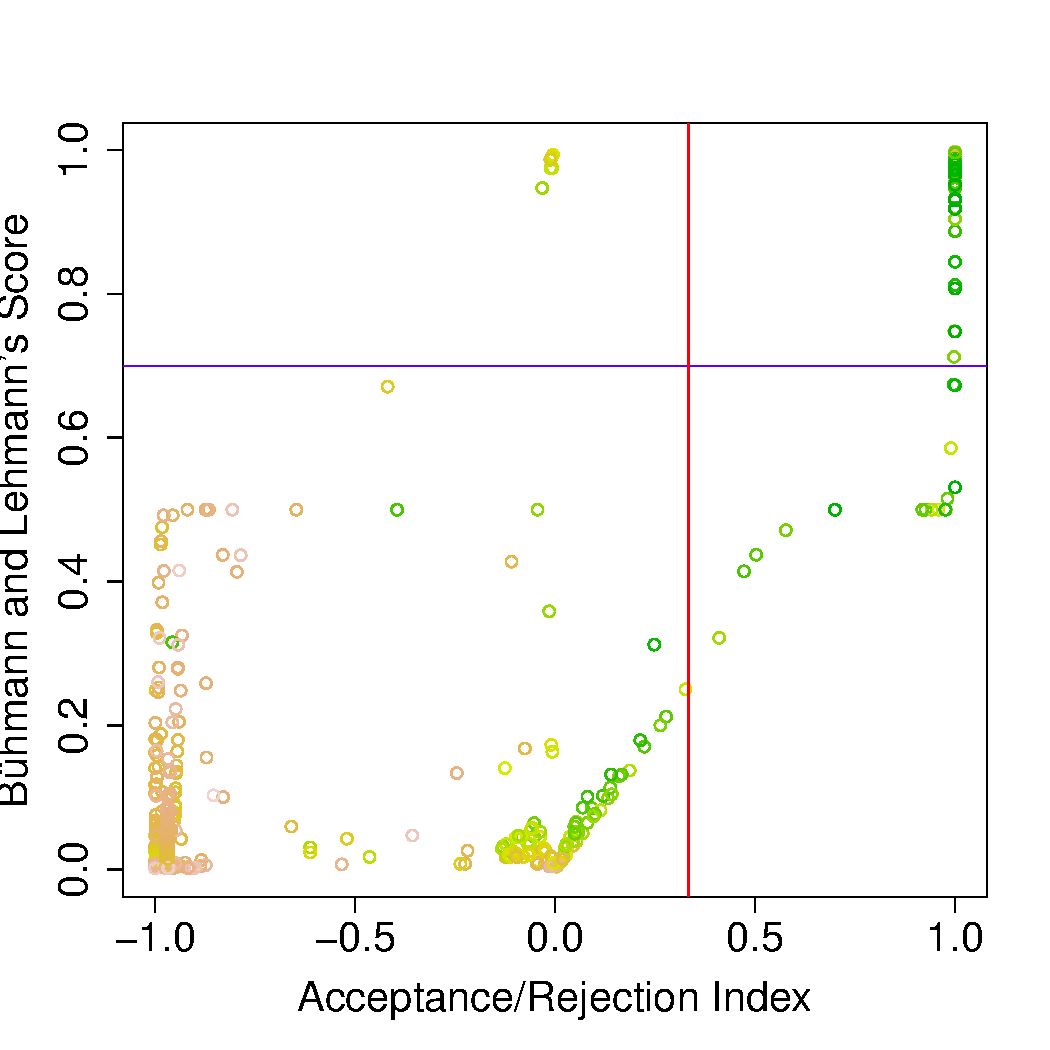
\includegraphics[height=\plotheight]{ARI-BLS}
\end{center}
\caption{A comparison of the acceptance/rejection index and the probability-based
  score used in~\cite{BuehmannLehmann2012} on axioms tested without time capping.
  The vertical red line shows the acceptance threshold $\mathrm{ARI}(\phi)>1/3$;
  the horizontal blue line the acceptance threshold of 0.7 for the probabilistic score.}
\label{fig:ARI-BLS}
\end{figure}

The improvement in accuracy of the possibilistic score, however, comes at a very high cost.
Testing a single axiom against an RDF dataset of the size of DBpedia can take
as little as a few milliseconds in some cases, but in many cases it can even take
days on a powerful workstation. The circles representing the axioms in Figure~\ref{fig:ARI-BLS}
are colored using a ``terrain'' palette based on the test time: green represents
the short times, rosish brown the longest times. The color scale is logarithmic.
A way to speed up testing is badly needed, lest the method we propose be practically useless.
Fortunately, a closer analysis of the time taken to test different axioms
pinpoints some regularities. We will base this analysis on the above-mentioned results.
Altogether, a staggering 24,151,287,253 ms (a little more than 279 days and a half)
of CPU time have had to be spent to gather them.

Testing \texttt{SubClassOf} axioms requires executing at least three SPARQL queries,
according to Algorithm~\ref{algo:uncapped-axiom-test}, which is a plain implementation
of the scoring scheme described in the previous sections.

\begin{algorithm}
\caption{Test a \texttt{SubClassOf} axiom\hfill\break
  (plain version, without time cap).}\label{algo:uncapped-axiom-test}
\begin{algorithmic}[1]
  \REQUIRE $\phi$, an axiom of the form $\mbox{\tt SubClassOf}(C\ D)$;
  \ENSURE $\Pi(\phi)$, $N(\phi)$, a list of confirmations, and a list of counterexamples.
  \STATE Compute $u_\phi$ using the query in Equation~\ref{eq:query-refc};
  \STATE compute $u^+_\phi$ using the query in Equation~\ref{eq:query-conf};
  \IF{$0 < u^+_\phi \leq 100$}
    \STATE query a list of confirmations;
  \ENDIF
  \IF{$u^+_\phi < u_\phi$}
    \STATE compute $u^-_\phi$ using the query in Equation~\ref{eq:query-expt};\label{line:count-expt}
    \IF{$0 < u^-_\phi \leq 100$}
      \STATE query a list of counterexamples;
    \ENDIF
  \ELSE
    \STATE $u^-_\phi \leftarrow 0$;
  \ENDIF
  \STATE compute $\Pi(\phi)$ using Equation~\ref{eq:possibility};
  \STATE compute $N(\phi)$ using Equation~\ref{eq:necessity}.
\end{algorithmic}
\end{algorithm}

Of these, the query in Equation~\ref{eq:query-expt}, to count the number of counterexamples,
is where most CPU time is spent, order of magnitudes more than in the other queries taken as a whole.
The reason of this resides in the use of the \texttt{FILTER NOT EXISTS} clause
in the $Q(\neg D, \mbox{\tt ?x})$ graph pattern (see Equation~\ref{eq:approx-open-world-negation}).
This approximation of an open-world semantics is a critical ingredient of our
scoring heuristics and cannot be dispensed with.

Now, if we denote $T(\phi)$ the time it takes to test an axiom $\phi$ and we plot
$T(\phi)$ as a function of its score, $\mathrm{ARI}(\phi)$ (see Figure~\ref{fig:time-ARI}),
a rather striking pattern emerges: all axioms $\phi$ having a positive ARI
(thus $\Pi(\phi) = 1$ and $N(\phi) > 0$) have a very small $T(\phi)$.
$N(\phi) > 0$ means no counterexamples could be found ($u^-_\phi = 0$)
and some confirmations have been found ($u^+_\phi > 0$).
For axioms having an ARI around zero or negative, $T(\phi)$ may vary widely:
from Figure~\ref{fig:time-ARI}, it appears that the range of this variation
increases the more $ARI(\phi)$ approaches $-1$.
The relation between $T(\phi)$ and $\mathrm{ARI}(\phi)$ is probably more complex,
but for our purposes we may describe it by saying that
$T(\phi) = O\left((1 + \mathrm{ARI}(\phi))^{-1}\right)$ or, perhaps,
$T(\phi) = O\left(\exp(-\mathrm{ARI}(\phi))\right)$.

\begin{figure}[t]
\begin{center}
  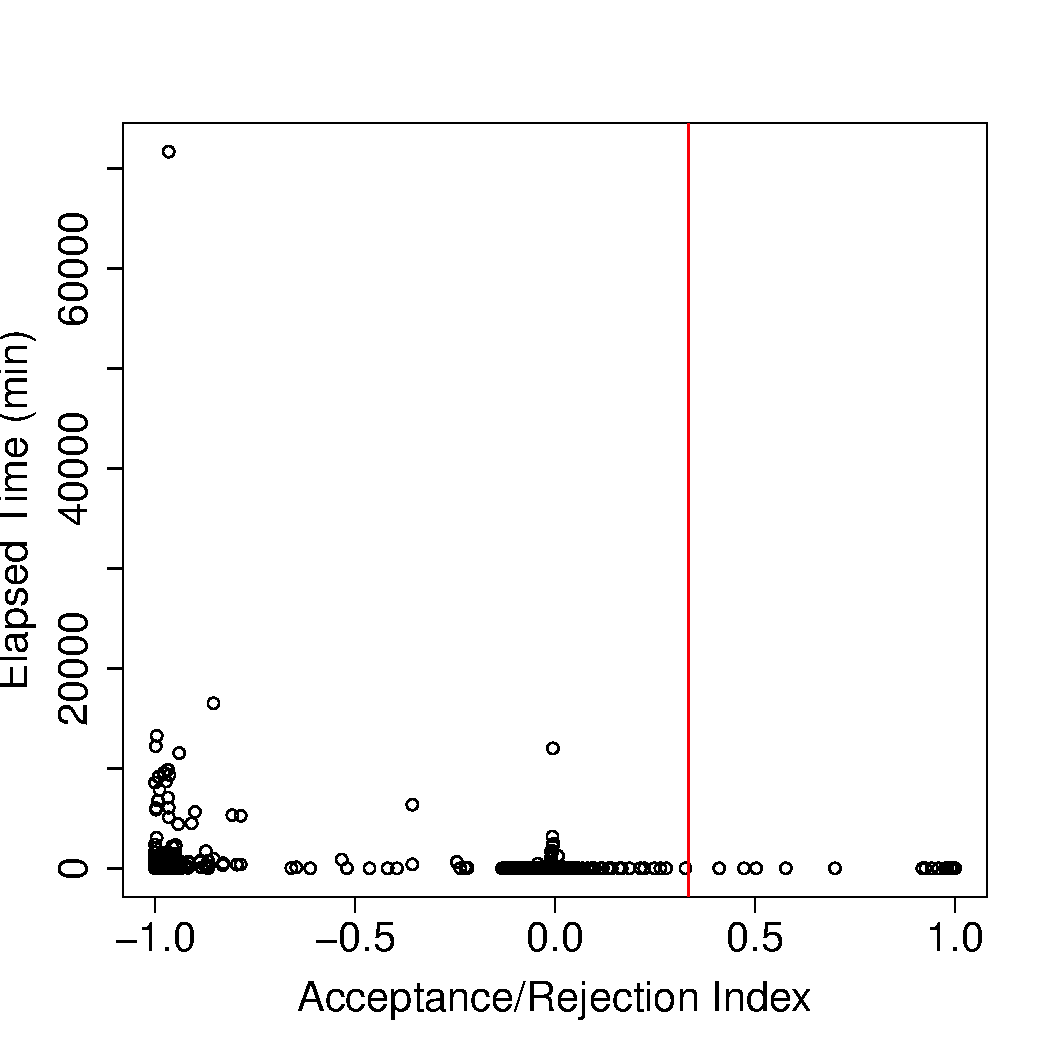
\includegraphics[height=\plotheight]{time-ARI}
\end{center}
\caption{Plot of the time taken for testing the systematically generated
  \textsf{SubClassOf} axioms without time capping as a function of ARI.
  The vertical red line shows the acceptance threshold $\mathrm{ARI}(\phi)>1/3$.}
\label{fig:time-ARI}
\end{figure}

Be that as it may, an axiom which takes too long to test will likely end up
being rejected. This naturally suggests that a strategy to speed up the test might
be to cap the time allowed to execute the query on Line~\ref{line:count-expt}
of Algorithm~\ref{algo:uncapped-axiom-test} and to reject an axiom if the test
runs out of time.

The question now is: how much time should we allow in order to be reasonably sure
we are not throwing the baby out with the bathwater, while avoiding to waste
time on hopeless tests?
Knowing the relation between the axiom's score and $T(\phi)$ is of little help,
since we do not have $\mathrm{ARI}(\phi)$ before testing $\phi$. However,
studying the elapsed times for axioms that ended up being accepted
(the $\phi$ such that $\mathrm{ARI}(\phi) > 1/3$)
we observed that the time it takes to test a \textsf{SubClassOf} axiom of the form
$C \sqsubseteq D$ tends to be proportional to the product of $u_{C \sqsubseteq D}$,
its support (which is, according to Equation~\ref{eq:query-refc},
equal to the cardinality of $[Q(C, \mbox{\tt ?x})]$)
and the number of classes that have at least a known instance in common with $C$,
which we will denote as \VAR{nic} (for ``number of intersecting classes'').
Since such product may be used to predict the time testing a valid axiom will take,
we will call it the \emph{time predictor} of an axiom, defined, in the case
of \textsf{SubClassOf} axioms, as
\begin{equation}\label{eq:time-predictor}
  \mathrm{TP}(C \sqsubseteq D) = u_{C \sqsubseteq D} \cdot
  \|\{A: [Q(C, x)] \cap [Q(A, x)] \neq \emptyset \}\|,
\end{equation}
where $A$ represents an atomic class expression.
Figure~\ref{fig:time-tp-acc} plots the test time of accepted axioms versus the
value of their time predictor, as well as the linear regression of the maximum time
for each value of the time predictor. We notice that a line having the same
slope $b$ as the regression line and an intercept $a = 2$ dominates all the
test times. This is a good candidate for the time out we are looking for.

\begin{figure}[t]
\begin{center}
    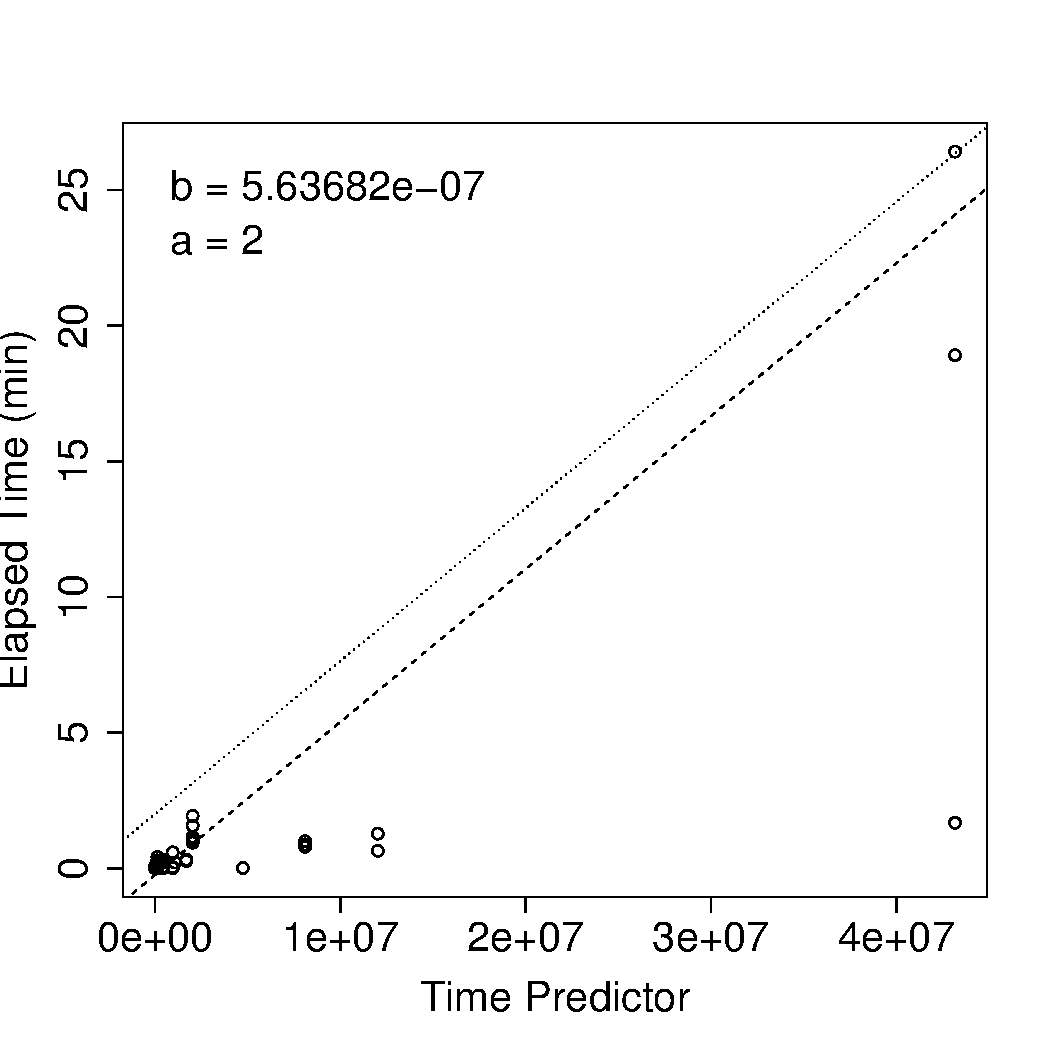
\includegraphics[height=\plotheight]{time-tp-acc}
\end{center}
\caption{Plot of the time taken to test the axioms that were accepted, without time capping,
  as a function of the time predictor. The dashed line shows the linear regression of the
  data points, while the dotted line is the strictest time-out having the same slope $b$
  and dominating all data points.}
\label{fig:time-tp-acc}
\end{figure}

Figure~\ref{fig:ratio-ARI} is a plot of the ratio of the elapsed time for testing axioms
to their time predictor. This diagram clearly shows that this ratio is very small for
accepted axioms (on the right of the acceptance threshold, shown as a red vertical line in the figure),
while it may soar to large values for ARIs around 0 and $-1$.

\begin{figure}[t]
\begin{center}
  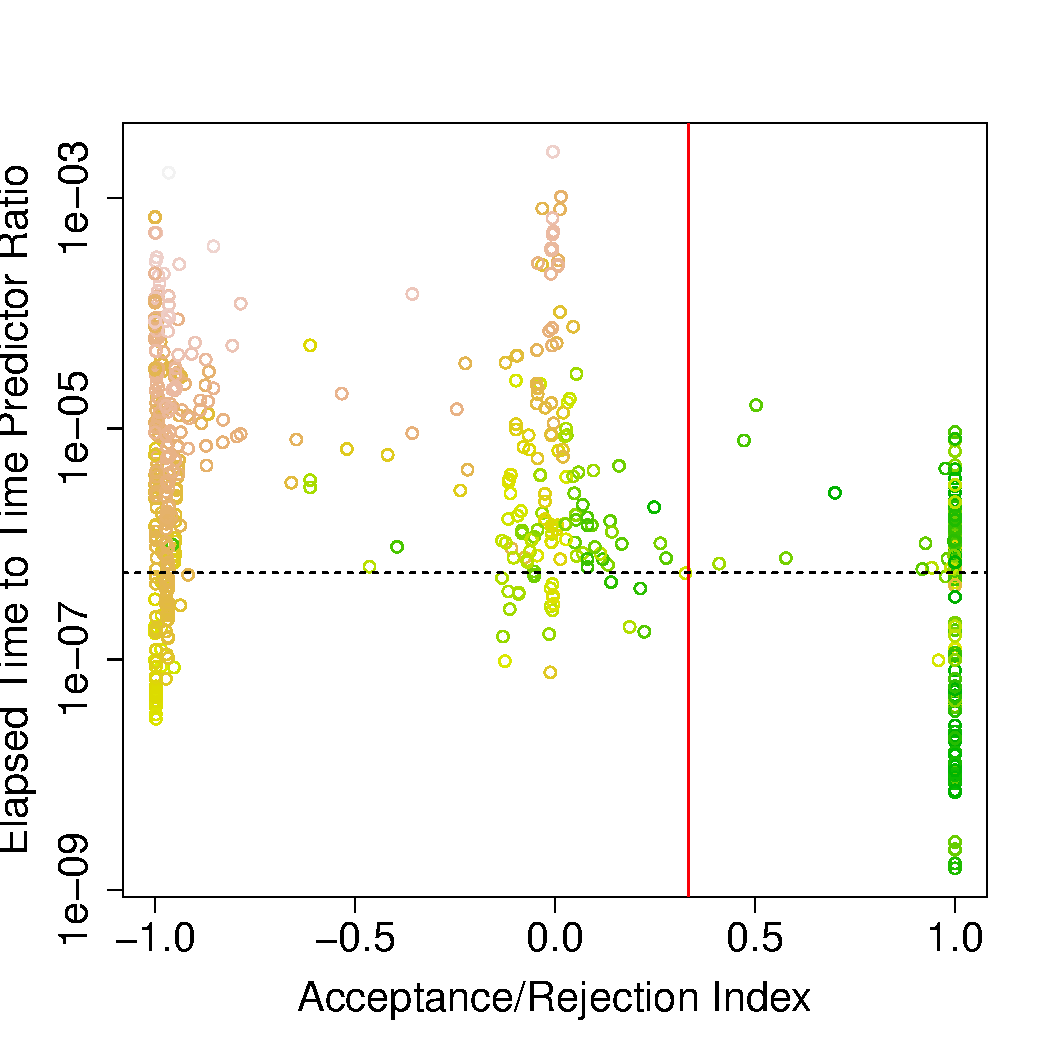
\includegraphics[height=\plotheight]{ratio-ARI}
\end{center}
\caption{Ratio of the time taken to test the axioms to the time predictor
  as a function of their acceptance-rejection index without time capping.
  The vertical red line shows the acceptance threshold $\mathrm{ARI}(\phi)>1/3$;
  the horizontal dashed line corresponds to the slope of the regression line
  of Figure~\ref{fig:time-tp-acc} ($b$ coefficient).}
\label{fig:ratio-ARI}
\end{figure}

The time predictor only depends on the subclass (i.e., the left-hand side)
of a \textsf{SubClassOf} axiom. If we compute the
time predictor for all the classes of DBpedia and we sort them by increasing value
of their time predictor, we get the diagram shown in Figure~\ref{fig:tp}.
The $y$-axis of the diagram is in logarithmic scale and we can observe that
the value of the time predictor increases by more than seven orders of magnitude
as we go from the least to the most time-consuming axioms.
This suggests that, in order to maximize the number of axioms tested,
one might begin by the less time-consuming axioms, whose number is large,
and leave the more time-consuming axioms, whose number is small, to the end.

\begin{figure}[t]
\begin{center}
  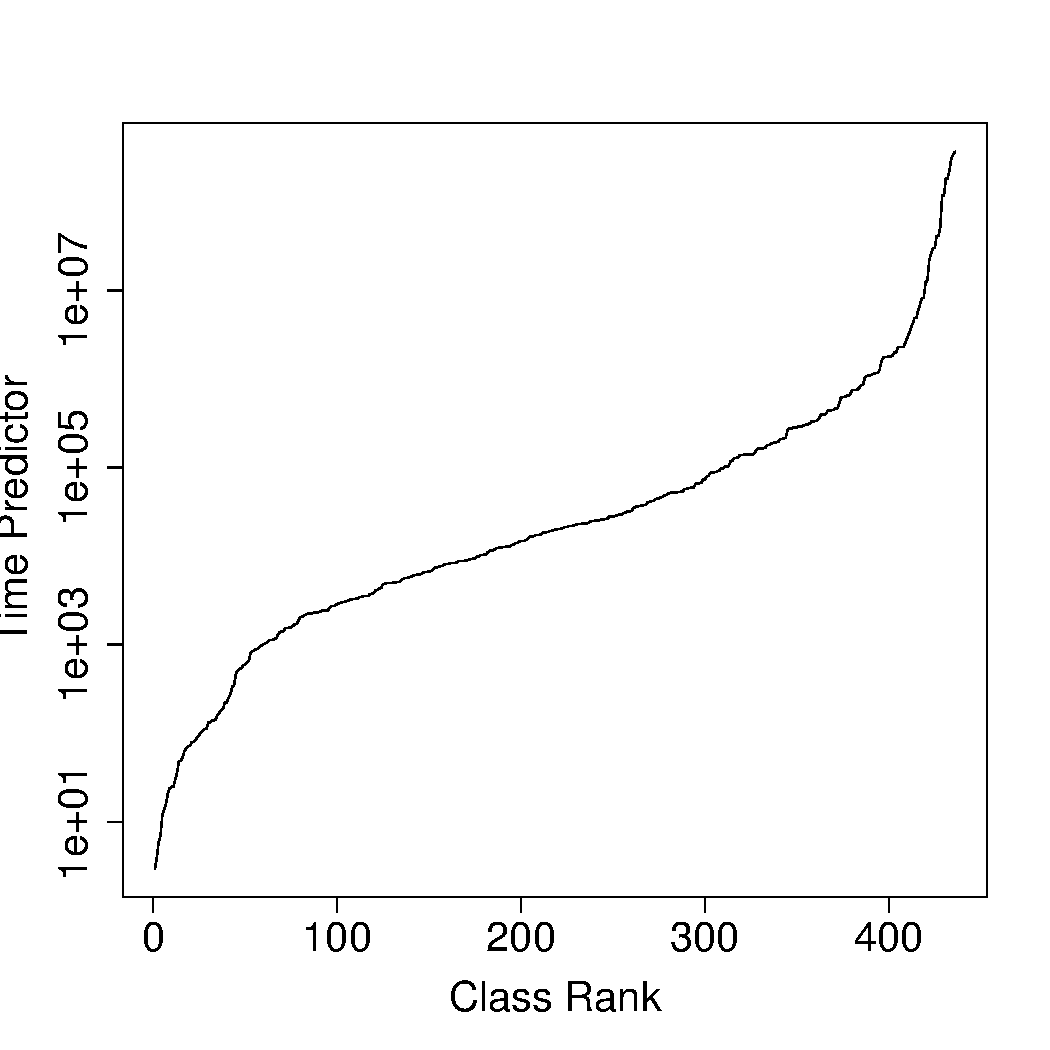
\includegraphics[height=\plotheight]{tp}
\end{center}
\caption{Plot of the time predictor for all the classes of DBpedia as a function of
  their rank when sorted by increasing value of the time predictor.}
\label{fig:tp}
\end{figure}


\subsection{Heuristics based on Time Capping}

We define two heuristics based on the analysis of the previous section.
\begin{itemize}

\item We dynamically time-cap the SPARQL queries to compute the ARI of a candidate axiom
by a time out defined as
\begin{equation}\label{eq:time-cap}
  t_{\max}(\phi) = a + b\cdot\mathrm{TP}(\phi),
\end{equation}
where $b$ is the slope of the regression line of the maximum times observed
for each value of the time predictor and the intercept $a$ is large enough to include,
below the time out, all the accepted axioms in the set of the axioms tested without time cap;
we then interrupt the test of any $\phi$ that takes longer than $t_{\max}(\phi)$
and reject it, $\phi$ being highly likely to get a negative ARI and be rejected anyway.
This heuristics yields a new version of the axiom testing procedure, which is
summarized by Algorithm~\ref{algo:time-capped-axiom-test}.

\item We construct candidate axioms of the form $C \sqsubseteq D$, by considering
the subclasses $C$ in increasing order of time predictor.
This enables us to maximize the number of tested and accepted axioms in a given time period.

\end{itemize}


\begin{algorithm}
\caption{Test a \texttt{SubClassOf} axiom\hfill\break
  (time-capped version).}\label{algo:time-capped-axiom-test}
\renewcommand{\algorithmicfor}{\textbf{waiting up to}}
\begin{algorithmic}[1]
  \REQUIRE $\phi$, an axiom of the form $\mbox{\tt SubClassOf}(C\ D)$;\\
    $a$, $b$, the coefficients of the linear time cap equation.
  \ENSURE $\Pi(\phi)$, $N(\phi)$, a list of confirmations, and a list of counterexamples.
  \STATE Compute $u_\phi$ using the query in Equation~\ref{eq:query-refc};
  \STATE Compute \VAR{nic} using query\\
    \texttt{SELECT (count(DISTINCT ?A) AS ?nic)}\\
    \texttt{WHERE} \{ $Q(C, \mbox{\tt ?x})$\quad \texttt{?x a ?A .} \}
  \STATE $\mathrm{TP}(\phi) \leftarrow u_\phi \cdot \VAR{nic}$;
  \STATE compute $u^+_\phi$ using the query in Equation~\ref{eq:query-conf};
  \IF{$0 < u^+_\phi \leq 100$}
    \STATE query a list of confirmations;
  \ENDIF
  \IF{$u^+_\phi < u_\phi$}
    \STATE $t_{\max}(\phi) \leftarrow a + b\cdot\mathrm{TP}(\phi)$
    \FOR{$t_{\max}(\phi)$ min}
      \STATE compute $u^-_\phi$ using the query in Equation~\ref{eq:query-expt};\label{line:count-expt}
    \ENDFOR
    \IF{\textbf{time-out}}
      \STATE $u^-_\phi \leftarrow u_\phi - u^+_\phi$;
    \ELSIF{$0 < u^-_\phi \leq 100$}
      \STATE query a list of counterexamples;
    \ENDIF
  \ELSE
    \STATE $u^-_\phi \leftarrow 0$;
  \ENDIF
  \STATE compute $\Pi(\phi)$ using Equation~\ref{eq:possibility};
  \STATE compute $N(\phi)$ using Equation~\ref{eq:necessity}.
\end{algorithmic}
\end{algorithm}

%In statistics, \emph{censoring} is when the value of a measurement or observation
%is not known for some sample points. A sample contains censored observations
%if the only information about some of the observations is that they are below
%or above a specified value.
%
% NIST/SEMATECH e-Handbook of Statistical Methods, http://www.itl.nist.gov/div898/handbook/, Jan 11, 2015
% http://www.itl.nist.gov/div898/handbook/apr/section1/apr131.htm
%
% Chapter 11, Analyzing Below Detection-limit data, from Millard, Dixon, and Neerchal, Environmental Statistics with R
% http://www.public.iastate.edu/~pdixon/stat505/Chapter%2011.pdf

%Here, we use this concept to refer to the fact that, when testing an OWL axiom,
%if one caps the time the test should take, the exact value of the score
%for the axiom whose test times out will not be known.
%From a statistical point of view, this produces a random censoring,
%because both the number of censored observations and the censoring levels
%are random outcome.


\section{Evaluation}% on \texttt{SubClassOf} Axiom Testing
\label{evaluation}

\subsection{Experimental Protocol}

We evaluated the proposed dynamic time-capping heuristics summarized in
Algorithm~\ref{algo:time-capped-axiom-test}
by performing tests of subsumption
axioms using DBpedia 3.9 in English as the reference RDF fact repository.
In particular, to obtain comparability with~\cite{TettamanziFaronZuckerGandon2014ekaw},
we used a local dump of DBpedia English version 3.9, along with the DBpedia ontology, version 3.9.
This local dump of DBpedia, consisting of 812,546,748 RDF triples,
has been bulk-loaded into Jena TDB and a prototype
for performing axiom tests using the proposed method has been coded in Java,
using Jena ARQ and TDB to access the RDF repository.

We systematically generated and tested subsumption axioms
involving atomic classes only, according the following protocol:
for each of the 442 classes $C$ referred to in the RDF repository,
we construct all axioms of the form $C \sqsubseteq D$ such that $C$ and $D$
share at least one instance. Classes $D$ are obtained with query
\texttt{SELECT DISTINCT ?D WHERE} \{ $Q(C, \mbox{\tt ?x})$ \texttt{?x a ?D} \}.
In addition, we tested these axioms in increasing time-predictor order.
To determine the dynamic time cap according to Equation~\ref{eq:time-cap},
we used $a = 2$ and $b = 5.63682\cdot 10^{-7}$, on the basis of the
results previously collected using the plain implementation of the scoring scheme
without time cap summarized in Algorithm~\ref{algo:uncapped-axiom-test}.

All experiments have been performed on a Fujitsu CELSIUS workstation equipped
with twelve six-core Intel Xeon CPU E5-2630 v2 processors at 2.60GHz clock speed,
with 15,360 KB cache each, 128 GB RAM,
4 TB of disk space with a 128 GB SSD cache,
under the Ubuntu  12.04.4 LTS 64-bit operating system.
This is the same machine used for~\cite{TettamanziFaronZuckerGandon2014ekaw};
in both cases the running times reported refer to (user + system) CPU time
given by the \texttt{ru\_utime.tv\_sec} field of the structure returned by
the Linux system call \texttt{getrusage(RUSAGE\_SELF, \dots)};
as a consequence, the times are commensurable.


\subsection{Results}

\begin{figure}[t]
\begin{center}
<<<<<<< .mine
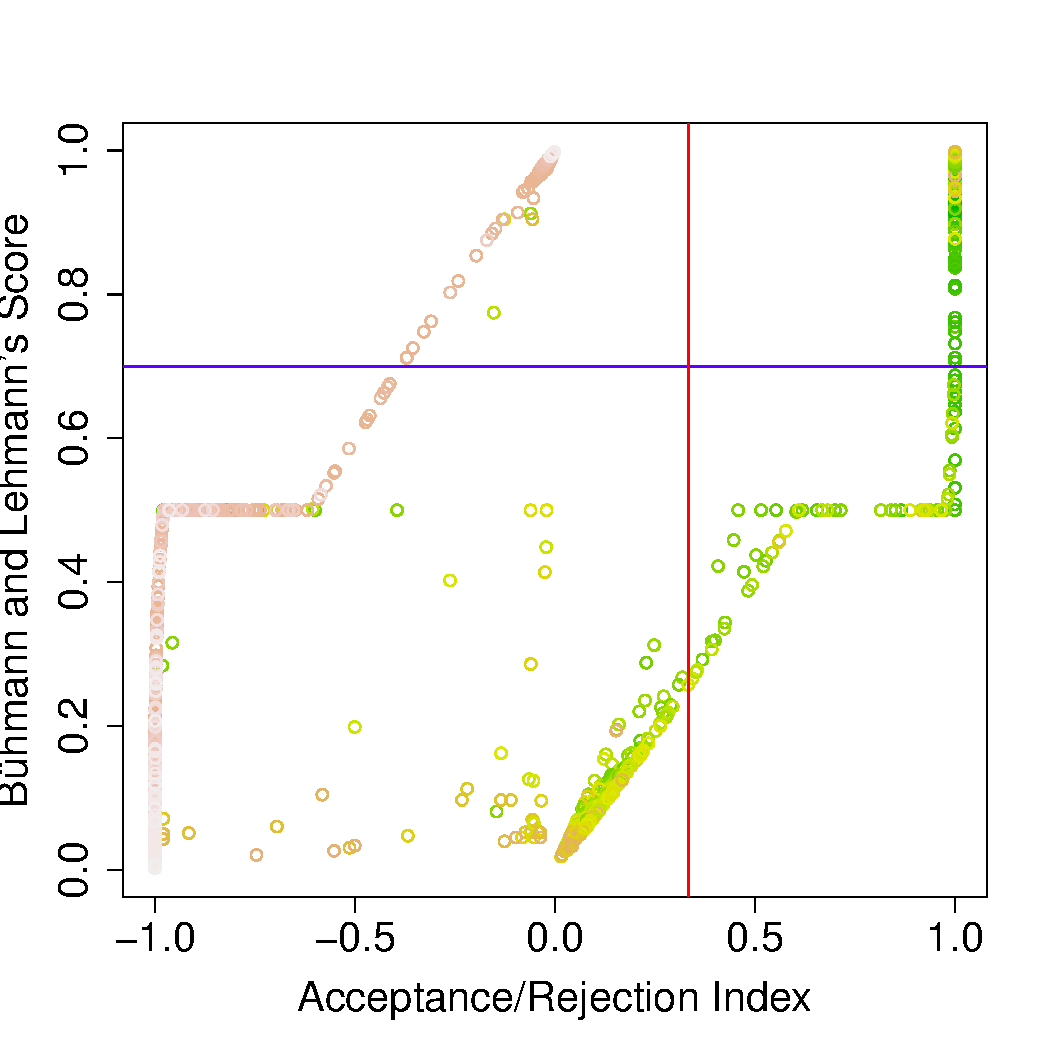
\includegraphics[height=\plotheight]{ARI-BLS-dtc}
=======
  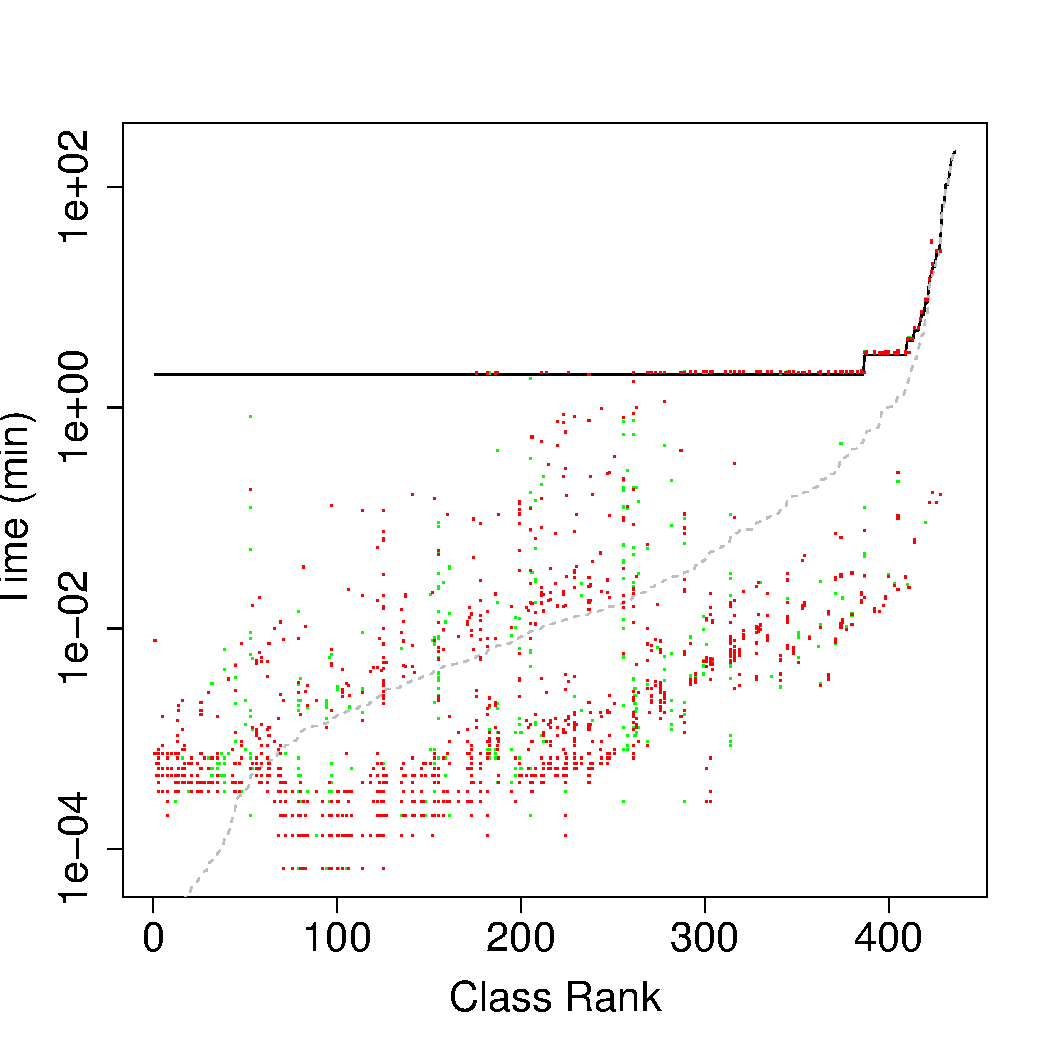
\includegraphics[height=\plotheight]{pred-and-actual-time}
\end{center}
\caption{Comparison of the actual testing time versus the computed time out
  as a function of the rank of an axiom's time predictor. Green dots represent
  accepted axioms and red dots rejected axioms. The gray dashed line shows the
  time as predicted by the time predictor (i.e., $\mathrm{TP}\cdot b$).}
\label{fig:pred-and-actual-time}
\end{figure}

\todo{Update according to the latest available results}
Thanks to the greatly reduced overhead of the dynamic time-capping heurustics,
we managed to test 3811 axioms at the time of writing (the experiment is still running).
Figure~\ref{fig:ARI-BLS-dtc} shows a summary of the results with a comparison
to the probabilistic score.

\begin{figure}[t]
\begin{center}
  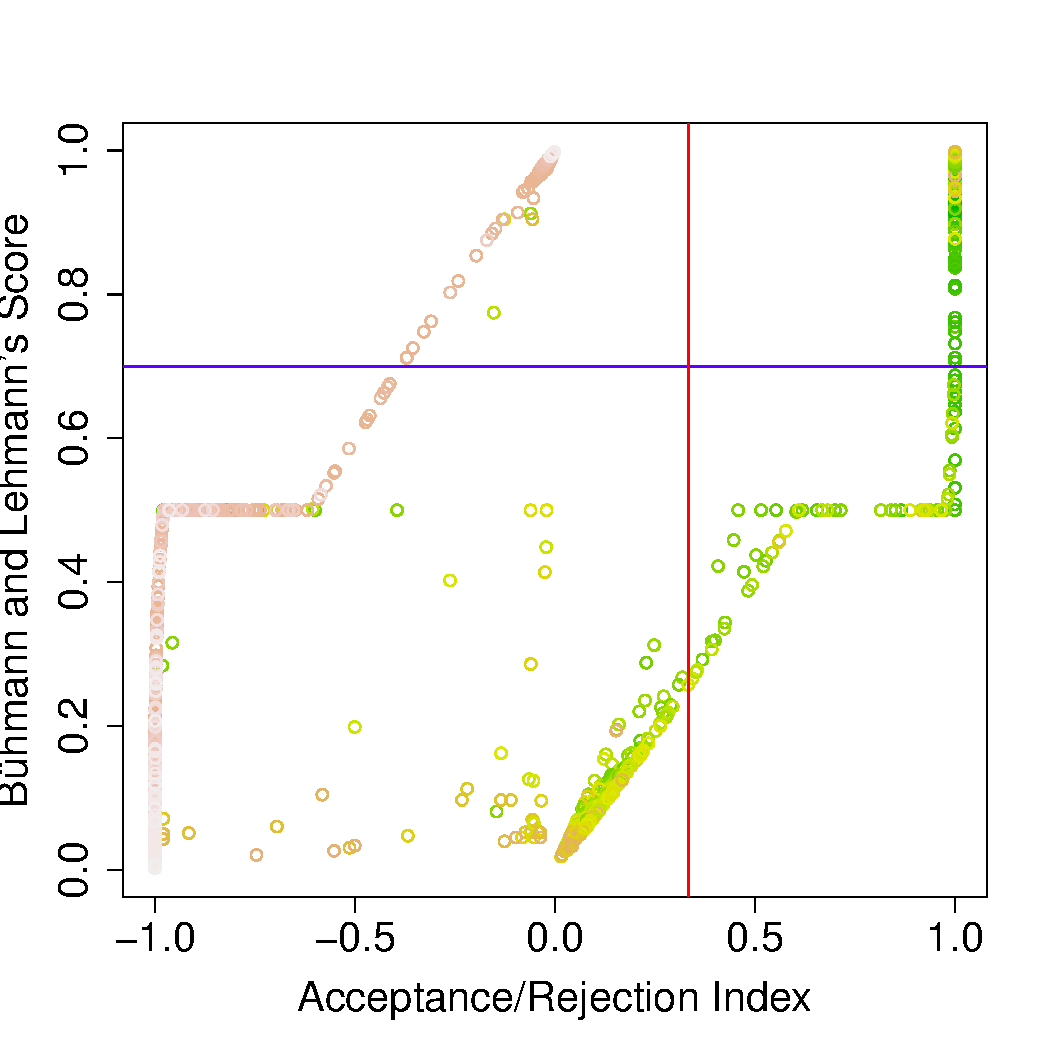
\includegraphics[height=\plotheight]{ARI-BLS-dtc}
>>>>>>> .r191
\end{center}
\caption{A comparison of the acceptance/rejection index and the probability-based
  score used in~\cite{BuehmannLehmann2012} on axioms tested with time capping.
  The vertical red line shows the acceptance threshold $\mathrm{ARI}(\phi)>1/3$;
  the horizontal blue line the acceptance threshold of 0.7 for the probabilistic score.}
\label{fig:ARI-BLS-dtc}
\end{figure}

\todo{FROM HERE ON, THE TEXT MUST BE STILL REVISED AND ADAPTED}

There are XXX axioms that were tested both with and without time capping;
the outcome of the test is different on just XXX of them,
namely
\dots
That represents an error rate of XXX\%. If we take into account the dramatic
improvement in terms of speed, this looks like a very reasonable price to pay
in terms of accuracy degradation. In addition, it should be observed that,
by construction, the errors are all in the same direction, i.e., some axioms
which should be accepted are in fact rejected: at least, this is a conservative
heuristics, since it does not generate false positives.

%\begin{figure}[t]
%\begin{center}
%  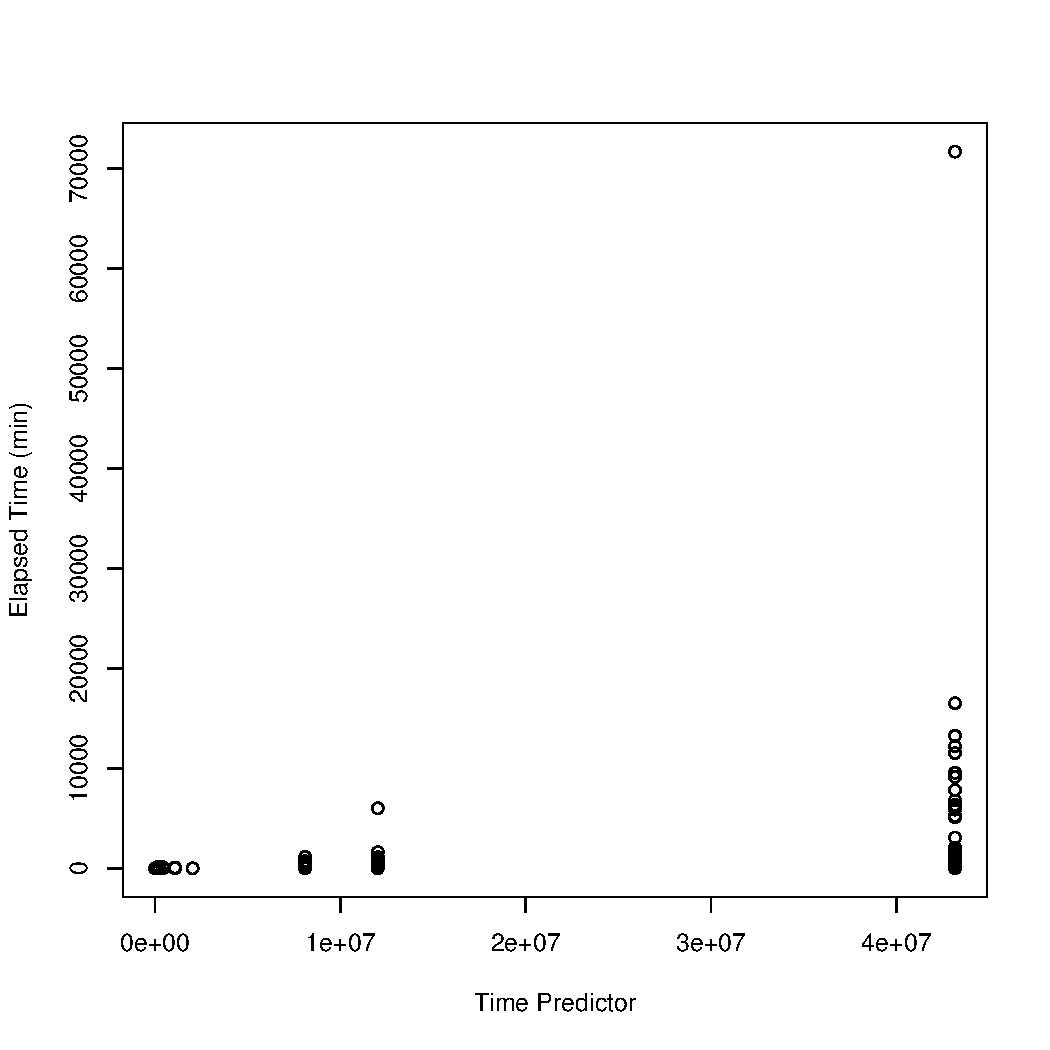
\includegraphics[height=\plotheight]{time-tp}
%\end{center}
%\caption{Plot of the time taken to test candidate axioms, without time capping,
%  as a function of the time predictor.}
%\label{fig:time-tp}
%\end{figure}


<<<<<<< .mine
Figure~\ref{fig:ratio-ARI} is a plot of the ratio of the elapsed time for testing axioms
to their time predictor. This diagram clearly shows that this ratio is very small for
accepted axioms (on the right of the acceptance threshold, shown as a red vertical line in the figure),
while it may soar to large values for ARIs around 0 and $-1$.

\begin{figure}[t]
\begin{center}
  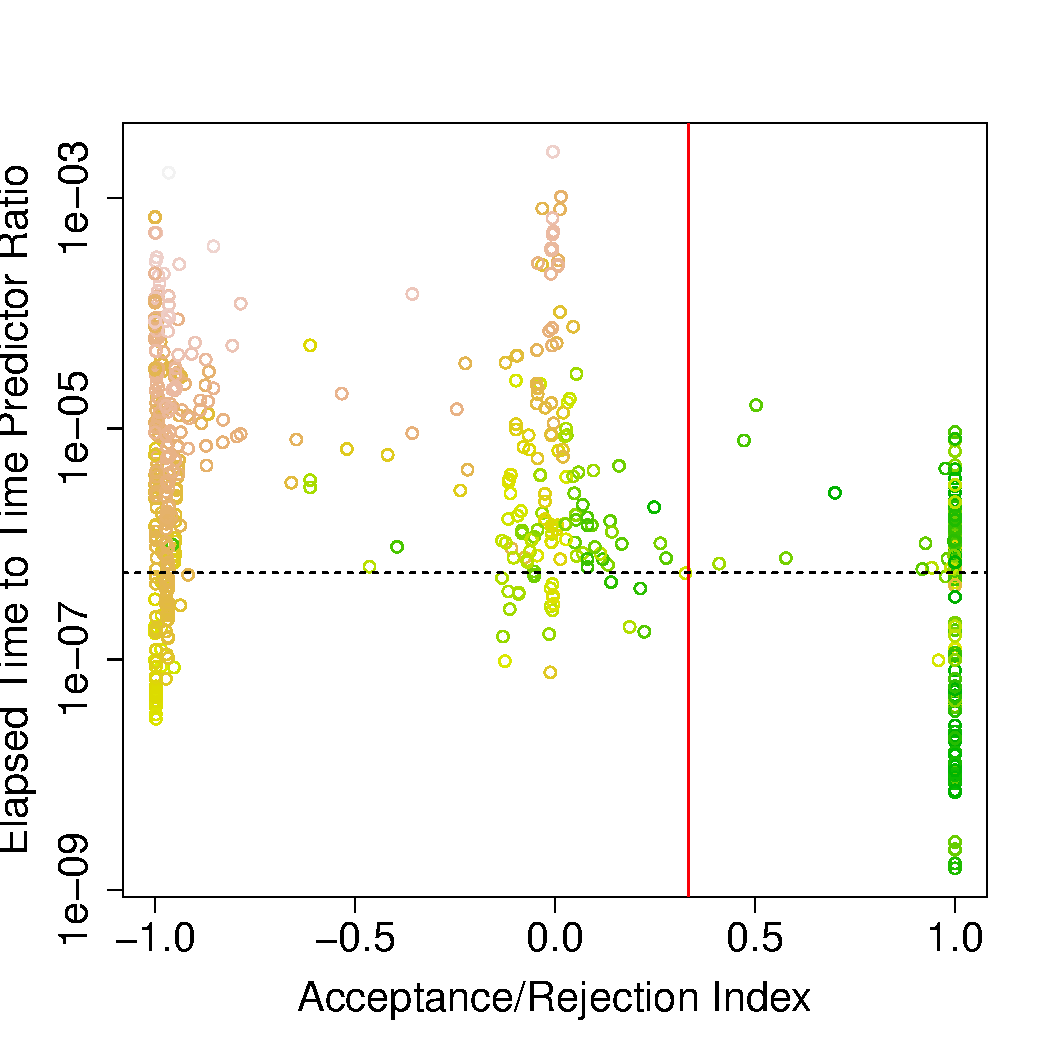
\includegraphics[height=\plotheight]{ratio-ARI}
\end{center}
\caption{Ratio of the time taken to test the axioms to the time predictor
  as a function of their acceptance-rejection index without time capping.
  The horizontal red line shows the acceptance threshold $\mathrm{ARI}(\phi)>1/3$.}
\label{fig:ratio-ARI}
\end{figure}


=======
>>>>>>> .r191
\section{Conclusion}

We have presented a possibilistic axiom scoring heuristics which is a viable
alternative to statistics-based heuristics. We have tested it by applying it to the
problem of testing \textsf{SubClassOf} axioms against the DBpedia database.
We have also proposed an additional heuristics to greatly reduce its computational
overhead, consisting of setting a dynamic time-out on the test of each axiom.

Our results strongly support the validity of our hypothesis
that it is possible to alleviate the computation of the ARI without loosing too much
in terms of accuracy.

In addition, a human evaluation of the axioms scored by the system shows that
most of the axioms accepted by mistake are inverted \textsf{subClassOf} relations between concepts (e.g. \textsf{dbo:Case} $\sqsubseteq$ \textsf{dbo:LegalCase} instead of \textsf{dbo:LegalCase} $\sqsubseteq$ \textsf{dbo:Case}). This occurs when counterexamples are missing (all instances of a class are instances of the other class too and the two axioms are positively scored).
Other mistakes are on axioms involving vague concepts (e.g., it seems that anything that can appear on a map could be typed with \textsf{gml:\_Feature} and therefore many classes should be subclasses of it, but it is not clear wether this is correct or not) or used in a more general sense thant it could be expected (e.g., \textsf{dbo:PokerPlayer} $\sqsubseteq$ \textsf{dbo:Athlete}; this is not really a mistake in the sense that there are several other such concepts involving \textsf{dbo:Athlete}).
Another example of mistakes on is the use of a concept in at least two senses, e.g \textsf{dbo:Library} designating both a building and an institution.
Other frequent mistakes are on axioms involving a concept both used as a zoological class name, a taxon, and therefore marked as subclass of \textsf{dbp:Species}, and as a set of animals, and therefore subclass of \textsf{dbo:Animal} and \textsf{dbo:Eukaryote}.
The same confusion between the instance level and the ontological level explain the results on axioms involving \textsf{skos:Concept}.
%TO DO: Eclaircir de quoi sont mes exemples: des axiomes qu'on a scorés exacts alors qu'ils ne le sont peut-être pas, ou bien des axioms scorés trop bas qui devraient être pris mais sur des concepts vagues ou bien des axiomes scorés négatifs qui ne devraient pas l'être. Je n'ai pas d'explication pour cette dernière catégorie.
 
%inverted subClassOf relations: between dbo:SportManager and SoccerManager, dbo:ClericalAdministrativeRegion and dbo:Diocese, 

%Place (dbo ou schema) sens vague
%dbo:Athlete axiomes ok avec ce concept pris au sens large

%pb de modélisation sur domaines de pointe: en biologie, en juridique (SupremeCourtOfTheUnitedStatesCase)

These considerations confirm the interest of using axiom scoring heuristics like ours
not only to learn axioms from the LOD, but also to drive the validation and debugging of ontologies and RDF datasets.

\bibliographystyle{abbrv}
\bibliography{../RDFMining}
%
% ACM needs 'a single self-contained file'!
%
%APPENDICES are optional
%\balancecolumns
\end{document}

